\documentclass[11pt,a4paper]{article}

\usepackage{style2017}
\usepackage{hyperref}

\hypersetup{
    colorlinks =false,
    linkcolor=blue,
   linkbordercolor = 1 0 0
}
\newcounter{numexo}
\setcellgapes{1pt}

\begin{document}



\begin{NSI}
{Exercice}{POO}
\end{NSI}


\addtocounter{numexo}{1}
\subsection*{\Large Exercice \thenumexo}
un site de vente en ligne propose des articles de bricolage à la vente. Pour chaque article, celui-ci a:
\begin{itemize}
\item une référence sous forme de chaine alpha-numérique;
\item une désignation sous forme de chaine de caractères;
\item un prix sous forme de nombre
\end{itemize}
On donne ci-dessous un exemple d'articles que l'on peut trouver sur le site:

\begin{center}
\begin{tabular}{*{3}{|C{4cm}}|}\hline
ref & désignation & prix \\\hline
P21 & perceuse & 99,50 \euro \\\hline
M07 & meuleuse & 45 \euro \\\hline
V33 & visseuse sans fil & 69,90 \euro \\\hline
\end{tabular}
\end{center}

\begin{enumerate}
\item Écrire la classe Article et son constructeur permettant de créer des objets pour les outils de bricolage.
\item Créer les trois objets du site présents dans le tableau ci-dessus.
\item Le prix d'un article peut varier notamment lorsqu'il est soldé. 

Écrire une méthode \textbf{solder} qui permet de modifier ce prix. Cette méthode prend en argument le pourcentage de réduction sous forme de nombre entier à appliquer. Elle renvoie le prix modifié de l'article.
\end{enumerate}

\addtocounter{numexo}{1}
\subsection*{\Large Exercice \thenumexo}
On définit l'objet Compte\_bancaire. On donne l'interface de notre objet :
\begin{itemize}
\item Attributs : solde et titulaire.
\item Méthodes : est\_positif, crediter, debiter, virer\_vers, afficher ou \_\_repr\_\_
\end{itemize}

\begin{enumerate}
\item Écrire son constructeur.
\item Écrire les différentes méthodes.
\item Tester en créant un compte bancaire \textbf{A} avec un solde de $1000$ euros et un compte bancaire \textbf{B} avec un solde bancaire de 200 euros.
\item Effectuer un virement de 300 de A vers B.
\item Interdire tout virement si le solde du compte est négatif.
\end{enumerate}


\addtocounter{numexo}{1}
\subsection*{\Large Exercice \thenumexo}
Les fractions sont des nombres dits rationnels de la forme $a/b$ ou $\dfrac{a}{b}$. Les nombres $a$ et $b$ sont des nombres entiers et $b$ est strictement positif.

On va définir une classe Fraction dans laquelle nous retrouverons différentes méthodes pour les calculs. La classe Fraction possède deux attributs : \textbf{num} et \textbf{denom}.


\begin{enumerate}
\item Écrire le constructeur de cette classe. On prendra en compte le dénominateur strictement positif.
\item Ajouter une méthode \_\_str\_\_ qui renvoie une chaine de caractères de la forme "a/b", ou simplement "a" lorsque le dénominateur vaut 1.
\item Ajouter des méthodes \_\_eq\_\_ et \_\_lt\_\_ qui reçoivent une deuxième fraction en argument et renvoient True si la première fraction représente un nombre égal ou un nombre strictement inférieur à la deuxième fraction.
\item Ajouter des méthodes \_\_add\_\_ et \_\_mul\_\_ qui reçoivent une deuxième fraction en argument et renvoient respectivement la somme et le produit des deux fractions.
\item Tester toutes ces opérations
\end{enumerate} 
\subsubsection*{En supplément:}
\begin{enumerate}
\item Ajouter des méthodes pour calculer la différence et le quotient de deux fractions. Ces méthodes existent en global.
\item S'assurer que les fractions sont toujours irréductibles.
\end{enumerate}


\addtocounter{numexo}{1}
\subsection*{\Large Exercice \thenumexo}
On va définir une classe Date pour représenter une date avec trois attributs jour, mois et annee.
\begin{enumerate}
\item Écrire son constructeur avec les paramètres j, m et a.
\item On peut créer une variable de classe qui sera utilisée dans la classe par différentes méthodes. L'appel de cette méthode se fera par \textbf{nom de la classe.variable}.\medskip

Créer une variable de classe mois de type liste contenant les douze mois de l'année. Cette variable sera accessible  avec l'appel Date.mois
\item Ajouter une méthode \_\_str\_\_ qui renvoie une chaine de caractères de la forme "11 novembre 1918". Tester l'affichage avec la commande \textbf{print}.
\item Ajouter une méthode \_\_lt\_\_ qui permet de déterminer si une date d1 est antérieure à une date d2 en écrivant d1 < d2. La tester.
\item \begin{enumerate}
\item Modifier le constructeur avec des valeurs par défaut initialisées au 1 janvier 2000.
\item Créer un objet Date, nommé \textbf{ddn}, sans paramètres. Vérifier que les attributs de \textbf{ddn} ont pour valeurs la date du 1 janvier 2000.
\item Modifier les attributs \textbf{ddn} avec les dates de votre anniversaire.
\end{enumerate} 
\item Dans la question précédente, vous avez remarqué qu'il est possible de modifier la valeur des attributs d'un objet. Cela peut poser des problèmes surtout lorsqu'on a des attributs dont les valeurs ne doivent pas être accessibles.\medskip

Il est possible d'interdire l'accès aux attributs en les cachant. Il suffit d'ajouter un double souligné devant le nom de l'attribut après self.
\begin{enumerate}
\item Modifier dans le constructeur les attributs jour, mois et annee pour qu'ils soient cachés. 

Penser aussi à modifier les méthodes qui les utilisent.
\item Vérifier qu'il n'est plus possible de modifier les valeurs d'une date une fois créée.
\end{enumerate}
\item Pour accéder aux attributs cachés et les modifier, on peut créer des méthodes particulières appelées accesseurs et mutateurs.

On définit pour l'attribut caché jour, l'accesseur get\_jour et le mutateur set\_jour de la manière suivante:
\begin{center}
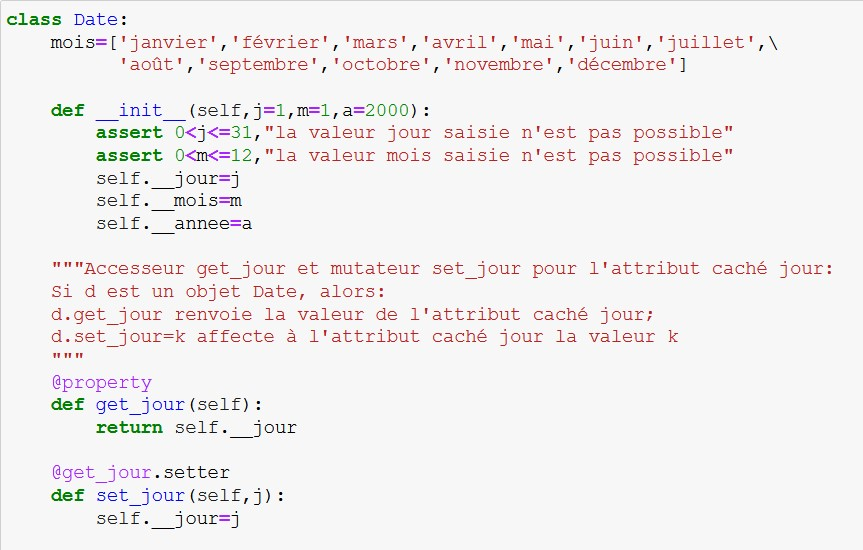
\includegraphics[scale=0.6]{img/poo1.eps}
\end{center}
\begin{enumerate}
\item Ajouter ces deux méthodes dans la classe Date et vérifier que vous pouvez afficher et modifier le jour d'une date.
\item Ajouter les accesseurs et les mutateurs pour le mois et l'année.
\item Vérifier, après avoir créé une date \textbf{ddn} sans paramètres, que vous pouvez la modifier par votre date de naissance.
\end{enumerate}
\end{enumerate}

\end{document}
